{\color{gray}\hrule}
\begin{center}
\section{Expérimentations}
\textbf{Dans cette section, nous verrons les expérimentations éffectuées et discuterons de leurs résulats.}
\bigskip
\end{center}
{\color{gray}\hrule}
\begin{multicols}{2}

Pour évaluer la justesse et l’efficacité de l’implémentation, il a fallu entraîner 
des architectures, ajuster leurs hyperparamètres, puis comparer les résultats obtenus avec 
ceux de Keras sur les mêmes architectures. \\

Le jeu de données MNIST a été choisi pour le premier test. Composé de 
60 000 images de chiffres manuscrits (de 0 à 9), il est l’un des jeux de données 
les plus connus pour les tâches de classification d’images. Chaque image mesure 
28x28 pixels et est en niveaux de gris. Ce jeu de données est particulièrement
populaire car il est simple à traiter et offre une grande qualité et quantité 
d’exemples, ce qui en fait une référence pour les premières expérimentations en 
apprentissage profond. \\

Cependant, afin d’augmenter la complexité des expérimentations, le jeu de données CIFAR-10\cite{CIFAR10} a également 
été utilisé. Il contient 60 000 images réparties en 10 classes (avions, voitures, oiseaux, chats, cerfs, 
chiens, grenouilles, chevaux, bateaux et camions). Les images sont des photographies sous échantillonnées, qui mesurent 32x32 pixels et qui sont en couleur 
(format RGB), ce qui les rend plus complexes à traiter que celles de MNIST. La diversité des classes et le manque de corrélation 
entre elles ajoutent également de la complexité à ce jeu de données. En ce qui concerne la qualité de ces dernières,
elle est comparable à celle de MNIST.

\subsection{Méthode}

Le protocole expérimental est le suivant :  \\


\textbf{Pré-traitement des données} Les données sont pré-traitées 
pour être compatibles avec les modèles.\\

\textbf{Création et évaluation d’architectures avec Melpy} Des architectures sont créées 
et entraînées avec différents hyperparamètres pour identifier celle qui offre 
la meilleure généralisation.\\

\textbf{Création et entraînement des architectures avec Keras} L'architecture
sélectionnée est ensuite entraînée avec Keras de manière similaire.

\textbf{Visualisation et interprétation des prédictions} On analyse les prédictions. 

\textbf{Comparaison des métriques finales} On compare les métriques finales d'une bibliothèque
avec celles de l'autres. \\

L’entraînement a été réalisé en utilisant un processeur Intel i5-12600K et 32 Go de RAM.


\subsection{Résultats et discussion}

\subsubsection{Pré-traitement des données}

Afin d’éviter des problèmes tels que \textit{Dead ReLU}, l’explosion des gradients 
ou encore la disparition des gradients, il est nécessaire de mettre les images à l’échelle.\\

Pour ce faire, nous commençons par normaliser les données, en les mettant sur une 
échelle allant de 0 à 1, puis nous les standardisons.\\

Enfin, les étiquettes doivent être encodées. Pour cela, nous utilisons l’encodeur One-Hot.\\

\subsubsection{Sélection du modèle}

\textbf{MNIST} \\

L'architecture sélectionnée pour MNIST est la suivante : \\

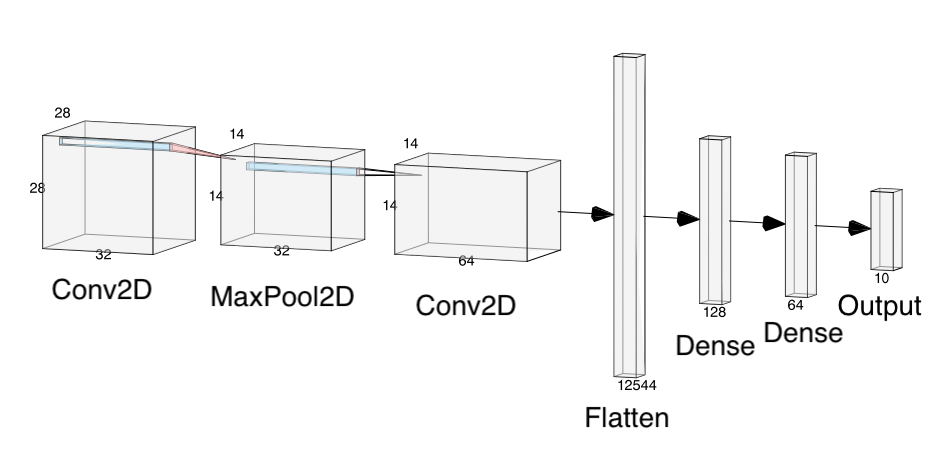
\includegraphics[width=\columnwidth]{images/mnist_nn.png}
\captionof{figure}{Réseau de neurones sélectionné pour MNIST}
\hfill\break

Comme illustré dans la Figure 10, le réseau de neurones commence par une couche de convolution qui 
génère 32 cartes de caractéristiques, suivie d’une couche de pooling qui réduit leur taille de moitié.
Ensuite, une seconde couche de convolution produit 64 cartes de caractéristiques, ensuite aplaties pour alimenter 
un MLP composé de deux couches cachées : la première avec 128 neurones et la seconde avec 64 neurones. \\

Les couches cachées utilisent la fonction d’activation Leaky ReLU, tandis que la sortie 
applique une fonction Softmax. Pour optimiser l'architecture, l’algorithme Adaptive Momentum (Adam) a été utilisé pour minimiser 
la fonction de coût d’entropie croisée catégorielle (Categorical Cross-Entropy). \\

\textbf{CIFAR-10} \\

L'architecture sélectionnée pour CIFAR-10 est la suivante : \\

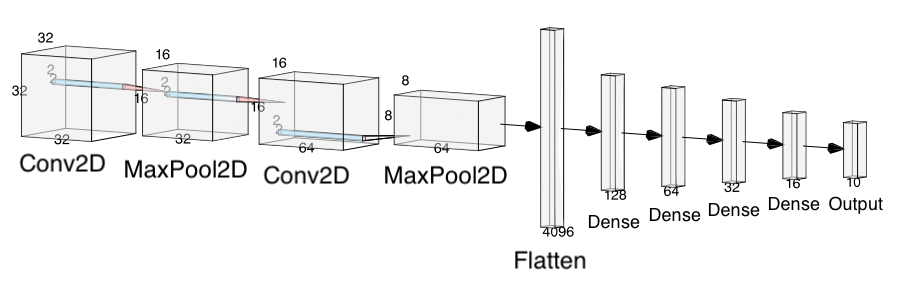
\includegraphics[width=\columnwidth]{images/cifar10_nn.png}
\captionof{figure}{Réseau de neurones sélectionné pour CIFAR-10}
\hfill\break

Comme illustré dans la Figure 11, le réseau de neurones se compose de deux couches de 
convolution et ne comporte aucune couche de pooling. Cette absence de pooling
s’explique par les expérimentations qui montrent qu’il est préférable de conserver 
les informations d’entrée intactes pour ce jeu de données. En effet, les photographies 
étant très petites, réduire leur taille risquerait d'écraser des caractéristiques importantes déjà 
difficiles à détecter. Les cartes de caractéristiques sont ensuite applaties pour alimenter
un MLP composé d'une couche cachée de 128 neurones. \\

La couche cachée utilise la fonction d’activation Leaky ReLU, 
tandis que la sortie est activée par la fonction Softmax. Pour optimiser l'architecture
on utilise l'algorithme Adaptive Momentum afin de minimiser la fonction de côut 
d'entropie croisée catégorielle. \\

Le choix a été fait sur les 6 entrainements suivants : \\

\scalebox{0.515}{
\begin{tabular}{l|c c c c c c c|}
    \cline{2-8}
                                   & $P$           & $D$                   & $e$       &$t/e$        & Lot     & $\gamma$             & $t$              \\
    \hline
    \multicolumn{1}{|l|}{$1$}      & 4 128 376            & $4C_{w}+2D_{w,b} = 6$        & 20            & 09min 50sec & 128     & $5^{-5}$             &03h 16min 59sec           \\
    \multicolumn{1}{|l|}{$2$}      & 2 107 146            & $2C_{w}+2D_{w,b} = 4$        & 20            & 15min 25sec & 128     & $1^{-5}$             &05h 48min 14sec           \\
    \multicolumn{1}{|l|}{$3$}      & 2 107 146            & $2C_{w}+2D_{w,b} = 4$        & 35            & 16min 07sec & 128     & $5^{-5}$             &09h 07min 21sec           \\
    \multicolumn{1}{|l|}{$4$}      & 2 107 146            & $2C_{w}+2D_{w,b} = 4$        & 50            & 08min 08sec & 256     & $5^{-5}$             &06h 50min 36sec          \\
    \multicolumn{1}{|l|}{$5$}      & 2 117 863            & $2C_{w}+2D_{w,b} = 4$        & 100           & 10min 30sec & 128     & $5^{-5}$             &17h 26min 00sec           \\
    \multicolumn{1}{|l|}{$6$}      & 2 107 242            & $2C_{w,b}+2D_{w,b} = 4$      & 50            & 12min 13sec & 64      & $5^{-6}$             &07h 08min 29sec           \\
    \hline
\end{tabular}}
\captionof{table}{Entrainements éffectués sur CIFAR-10 avec Melpy} \\

{\scriptsize
$P$ étant le nombre de paramètres dans l'architecture\\

$D$ étant la prodondeur de l'architecture avec $C$ une couche de convolution, D une couche entièrement connectée, $w$ l'utilisation de poids et $b$ l'utilisation de biais \\

$e$ étant le nombre d'époques passés pour entrainer l'architecture \\

$Lot$ étant le nombre d'entrées entrainées sur une passe avant et arrière \\

$\gamma$ étant le taux d'apprentissage utilisé dans l'algorithme d'optimisation \\

$t$ étant le temps qu'il a fallu pour entrainer l'architecture \\

$t/e$ étant le temps passé en moyenne sur une époque \\
} \\

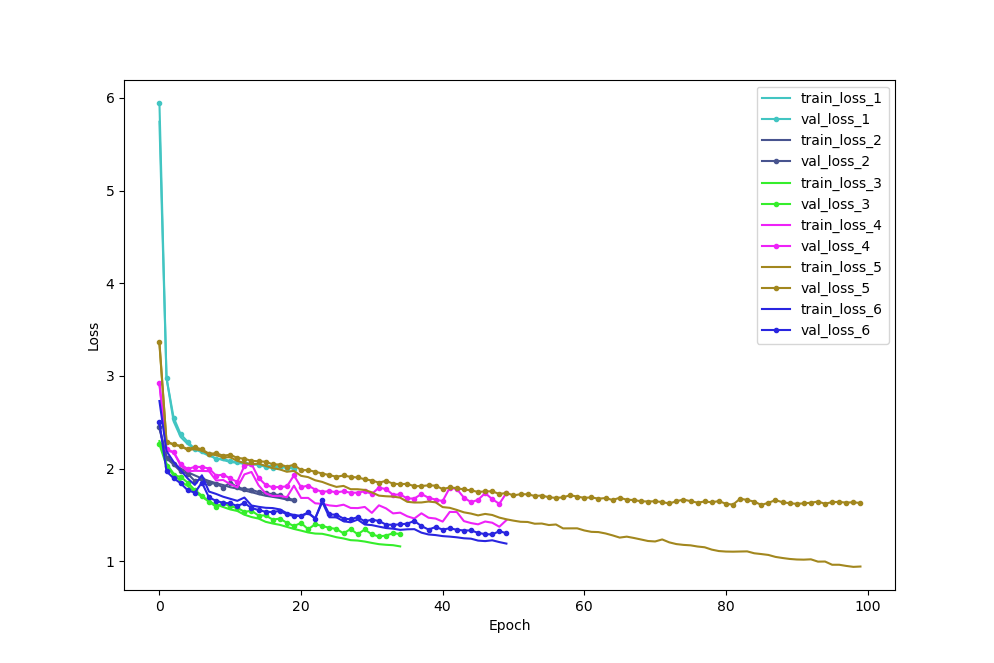
\includegraphics[width=\columnwidth]{images/cifar_10_losses.png}
\captionof{figure}{Les coûts calculés à la fin de chaque époque}
\hfill\break

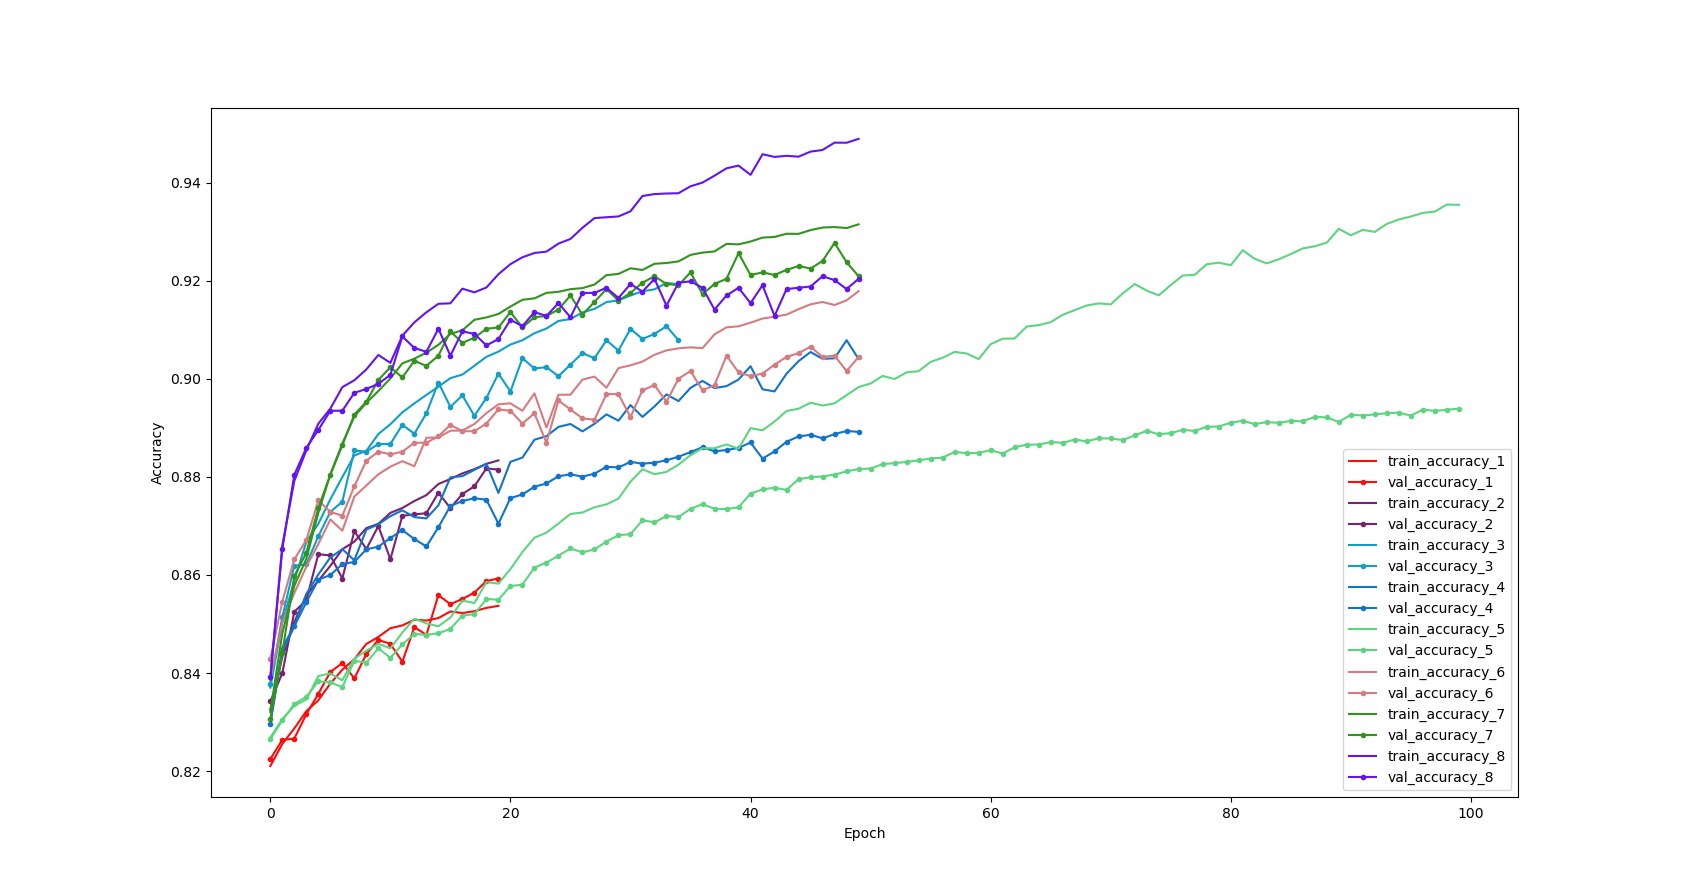
\includegraphics[width=\columnwidth]{images/cifar_10_accuracies.png}
\captionof{figure}{La précision des modèles calculées à la fin de chaque époque}
\hfill\break

Comme le montrent les Figures 12 et 13, les modèles 3, 6 et 4 se démarquent comme 
les plus performants. Parmi eux, c'est bien le modèle 6 qui a été retenu. Ce choix repose sur un 
compromis entre la qualité de sa généralisation, son temps d’entraînement réduit et 
son efficacité sur un faible nombre d’époques. Avec une petite taille de lot et un 
temps d’apprentissage relativement court, tout en ayant un nombre de paramètres 
légèrement supérieur, le modèle 6 offre un bon juste milieu entre les modèles. \\

On peut néanmoins noter les observations suivantes à partir de l'ensemble des entrainements :  
\begin{itemize}
    \item \textbf{Taille des lots} : Elle a un impact significatif sur le temps de calcul par époque ainsi que sur le nombre d’itérations nécessaires pour atteindre la convergence.  
    \item \textbf{Capacité de généralisation} : La taille des lots influence également la capacité du modèle à bien généraliser sur des données non vues.  
    \item \textbf{Nombre de paramètres} : Un modèle avec un grand nombre de paramètres peut rendre l’apprentissage plus instable et difficile, comme en témoignent les expériences présentées et mes observations lors 
    d'entrainements ayant subis les problèmes d'explosion ou disparition de gradients.
\end{itemize}



\subsubsection{Comparaison des résultats}

\end{multicols}